% Created 2014-10-17 vie 12:38
\documentclass[xcolor={usenames,svgnames,dvipsnames}]{beamer}
\usepackage[utf8]{inputenc}
\usepackage[T1]{fontenc}
\usepackage{fixltx2e}
\usepackage{graphicx}
\usepackage{longtable}
\usepackage{float}
\usepackage{wrapfig}
\usepackage{rotating}
\usepackage[normalem]{ulem}
\usepackage{amsmath}
\usepackage{textcomp}
\usepackage{marvosym}
\usepackage{wasysym}
\usepackage{amssymb}
\usepackage{hyperref}
\tolerance=1000
\usepackage{color}
\usepackage{listings}
\AtBeginSubsection[]{\begin{frame}[plain]\tableofcontents[currentsubsection,sectionstyle=show/shaded,subsectionstyle=show/shaded/hide]\end{frame}}
\lstset{keywordstyle=\color{blue}, commentstyle=\color{gray!90}, basicstyle=\ttfamily\small, columns=fullflexible, breaklines=true,linewidth=\textwidth, backgroundcolor=\color{gray!23}, basewidth={0.5em,0.4em}, literate={á}{{\'a}}1 {ñ}{{\~n}}1 {é}{{\'e}}1 {ó}{{\'o}}1 {º}{{\textordmasculine}}1}
\usepackage{mathpazo}
\hypersetup{colorlinks=true, linkcolor=Blue, urlcolor=Blue}
\usepackage{fancyvrb}
\DefineVerbatimEnvironment{verbatim}{Verbatim}{boxwidth=\textwidth, fontsize=\tiny, formatcom = {\color{black!70}}}
\usepackage{animate}
\usetheme{Goettingen}
\usecolortheme{rose}
\usefonttheme{serif}
\author{Oscar Perpiñán Lamigueiro}
\date{24 de Octubre de 2014}
\title{Visualización de datos raster}
\hypersetup{
  pdfkeywords={},
  pdfsubject={},
  pdfcreator={Emacs 24.3.1 (Org mode 8.2.7c)}}
\begin{document}

\maketitle

\section{Introducción}
\label{sec-1}

\subsection{Datos raster}
\label{sec-1-1}
\begin{frame}[label=sec-1-1-1]{Datos raster}
\begin{block}{}
Los datos raster consisten en una matriz de celdas cuadradas o
rectangulares organizadas en filas y columnas en la que cada celda
contiene un valor que representa información (temperatura, altitud,
uso del terreno). La localización geográfica de cada celda es
implícita, dependiendo del lugar que ocupa en la rejilla.
\end{block}
\end{frame}

\subsection{Paquete \texttt{raster}}
\label{sec-1-2}
\begin{frame}[fragile,label=sec-1-2-1]{\texttt{raster}}
 \begin{itemize}
\item Define funciones para crear, leer, manipular y escribir datos raster.
\item Implementa algebra raster y funciones de uso común en GIS.
\item Es capaz de trabajar con ficheros muy grandes trabajando en disco y procesando por lotes.
\item Clases:
\begin{itemize}
\item \texttt{RasterLayer}
\item \texttt{RasterBrick}
\item \texttt{RasterStack}
\end{itemize}
\end{itemize}

\begin{block}{Introduction to raster}
\url{http://cran.r-project.org/web/packages/raster/vignettes/Raster.pdf}
\end{block}
\end{frame}

\begin{frame}[fragile,label=sec-1-2-2]{Álgebra raster}
 \begin{itemize}
\item Funciones básicas: \texttt{abs}, \texttt{round}, \texttt{ceiling}, \texttt{floor}, \texttt{trunc},
\texttt{sqrt}, \texttt{log}, \texttt{log10}, \texttt{exp}, \texttt{cos}, \texttt{sin}, \texttt{max}, \texttt{min}, \texttt{range},
\texttt{prod}, \texttt{sum}, \texttt{any}, \texttt{all}.
\item Se pueden mezclar objetos \texttt{Raster*} con números.
\end{itemize}
\end{frame}

\begin{frame}[fragile,label=sec-1-2-3]{Funciones para modificar extensión}
 \begin{itemize}
\item \texttt{crop} extrae una región geográfica de un objeto \texttt{Raster*}
\item \texttt{trim} elimina las filas y columnas externas que sólo contienen \texttt{NA}.
\item \texttt{extend} añade filas y columnas con \texttt{NA}.
\item \texttt{merge} junta dos \texttt{Raster} en un nuevo objeto de mayor extensión.
\item \texttt{projectRaster} produce un nuevo \texttt{Raster*} con nuevo sistema de referencia geográfica.
\end{itemize}
\end{frame}
\begin{frame}[fragile,label=sec-1-2-4]{Funciones para modificar contenido}
 \begin{itemize}
\item \texttt{mask} elimina de una capa los valores que son \texttt{NA} en otra.
\item \texttt{cover} combina dos capas cogiendo los valores de la primera, excepto allí donde son \texttt{NA}.
\end{itemize}
\end{frame}
\begin{frame}[fragile,label=sec-1-2-5]{Funciones para combinar objetos.}
 \begin{itemize}
\item Con \texttt{overlay} se pueden combinar múltiples \texttt{Raster*} (por ejemplo, para multiplicarlos).
\item \texttt{calc} aplica una función en un objeto \texttt{Raster*}.
\item \texttt{stackApply} agrega capas de un \texttt{RasterStack} or \texttt{RasterBrick}.
\end{itemize}
\end{frame}
\begin{frame}[fragile,label=sec-1-2-6]{Funciones para extraer información}
 \begin{itemize}
\item \texttt{cut} y \texttt{reclassify} reemplazan rangos de valores por un único valor (de cuantitativo a cualitativo).
\item \texttt{zonal} aplica una función por zonas definidas por un determinado valor entero recogido en un \texttt{RasterLayer}.
\end{itemize}
\end{frame}
\subsection{Paquete \texttt{rasterVis}}
\label{sec-1-3}
\begin{frame}[fragile,label=sec-1-3-1]{\texttt{rasterVis}}
 \begin{block}{Métodos de visualización de datos raster basados en gráficos \texttt{grid}}
\end{block}
\begin{block}{\url{http://oscarperpinan.github.io/rastervis/}}
\end{block}
\end{frame}


\section{Datos Cuantitativos}
\label{sec-2}

\subsection{Datos}
\label{sec-2-1}

\begin{frame}[label=sec-2-1-1]{Radiación solar de CM SAF}
\begin{block}{CM SAF}
\begin{itemize}
\item \url{http://dx.doi.org/10.5676/EUM_SAF_CM/RAD_MVIRI/V001}
\item Promedio anual de la radiación global en el plano horizontal
(shortwave incoming solar radiation, SIS) en España durante 2008.
\end{itemize}
\end{block}
\end{frame}

\subsection{\texttt{levelplot}}
\label{sec-2-2}

\begin{frame}[fragile,label=sec-2-2-1]{Representación básica}
 \lstset{language=R,label= ,caption= ,numbers=none}
\begin{lstlisting}
  library(raster)
  library(rasterVis)
  SISav <- raster('data/SISav')
  levelplot(SISav)
\end{lstlisting}
\end{frame}

\begin{frame}[label=sec-2-2-2]{}
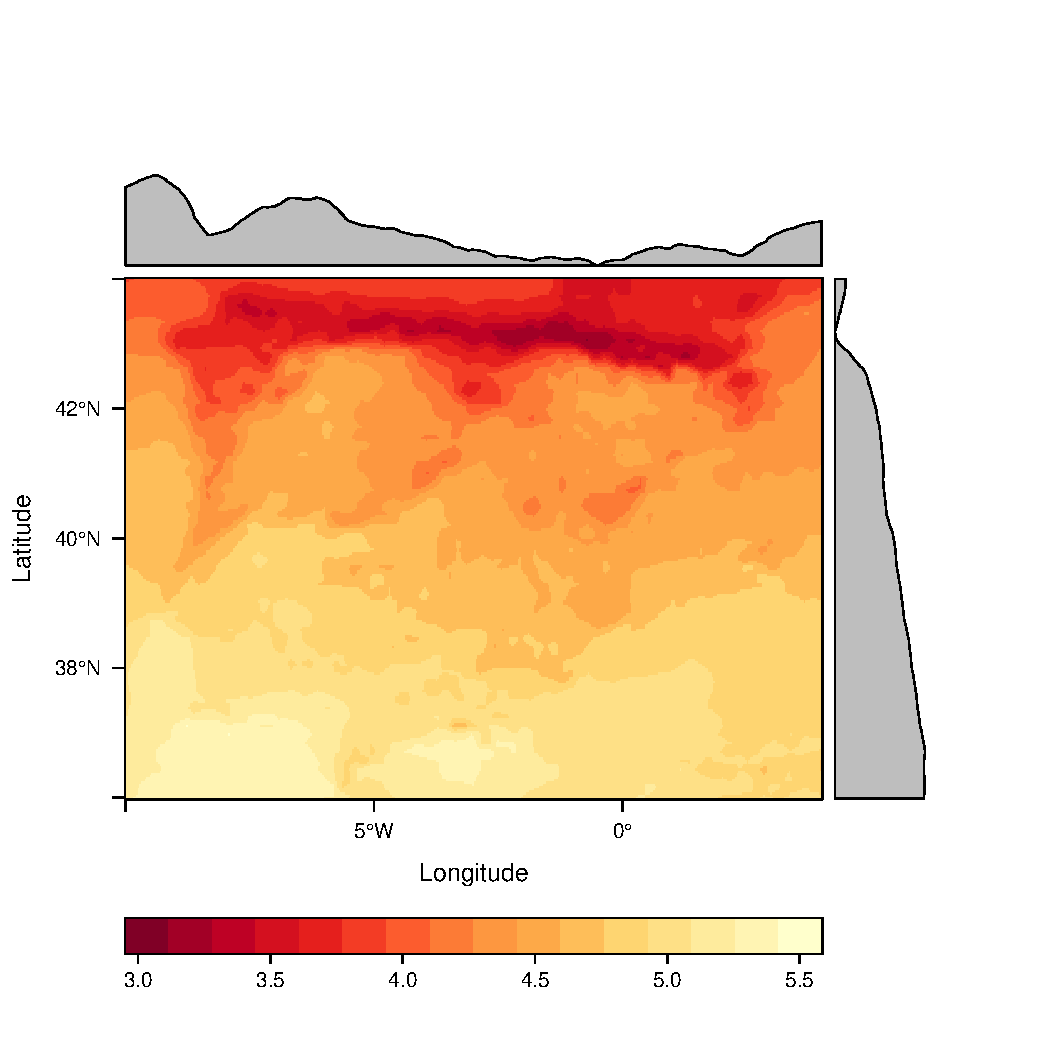
\includegraphics[width=.9\linewidth]{figs/leveplotSISavOrig.pdf}
\end{frame}

\begin{frame}[fragile,label=sec-2-2-3]{Fronteras}
 \lstset{language=R,label= ,caption= ,numbers=none}
\begin{lstlisting}
  library(maps)
  library(mapdata)
  library(maptools)
  
  ext <- as.vector(extent(SISav))
  boundaries <- map('worldHires',
                    xlim=ext[1:2], ylim=ext[3:4],
                    plot=FALSE)
  boundaries <- map2SpatialLines(boundaries,
                                 proj4string=CRS(projection(SISav)))
\end{lstlisting}
\end{frame}

\begin{frame}[fragile,label=sec-2-2-4]{}
 \lstset{language=R,label= ,caption= ,numbers=none}
\begin{lstlisting}
  levelplot(SISav) + layer(sp.lines(boundaries, lwd=0.5))
\end{lstlisting}

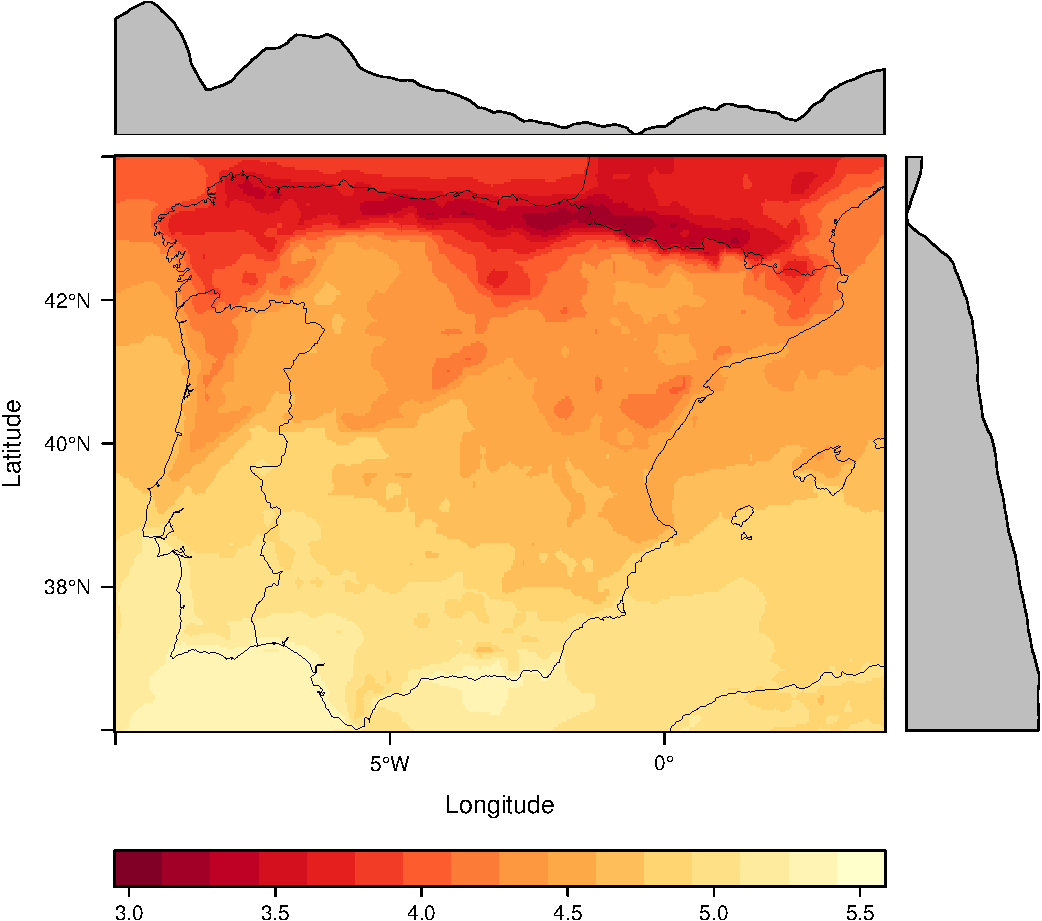
\includegraphics[width=.9\linewidth]{figs/leveplotSISavBoundaries.pdf}
\end{frame}

\subsection{Hill Shading}
\label{sec-2-3}
\begin{frame}[fragile,label=sec-2-3-1]{DEM}
 \begin{itemize}
\item Obtenemos un modelo digital del terreno (DEM) de DIVA-GIS.
\end{itemize}

\lstset{language=R,label= ,caption= ,numbers=none}
\begin{lstlisting}
  old <- setwd(tempdir())
  download.file('http://biogeo.ucdavis.edu/data/diva/msk_alt/ESP_msk_alt.zip', 'ESP_msk_alt.zip')
  unzip('ESP_msk_alt.zip', exdir='.')
  
  DEM <- raster('ESP_msk_alt')
\end{lstlisting}
\end{frame}

\begin{frame}[fragile,label=sec-2-3-2]{\texttt{terrain} y \texttt{hillShade}}
 \begin{itemize}
\item Calculamos el sombreado con \texttt{terrain} and \texttt{hillShade} de \texttt{raster}.
\end{itemize}

\lstset{language=R,label= ,caption= ,numbers=none}
\begin{lstlisting}
  slope <- terrain(DEM, 'slope')
  aspect <- terrain(DEM, 'aspect')
  hs <- hillShade(slope=slope, aspect=aspect,
                  angle=20, direction=30)
\end{lstlisting}

\lstset{language=R,label= ,caption= ,numbers=none}
\begin{lstlisting}
  setwd(old)
\end{lstlisting}
\end{frame}

\begin{frame}[fragile,label=sec-2-3-3]{Combinamos con transparencia}
 \begin{itemize}
\item Combinamos la capa de sombreado usando transparencia parcial
\end{itemize}

\lstset{language=R,label= ,caption= ,numbers=none}
\begin{lstlisting}
  ## hillShade theme: gray colors and semitransparency
  hsTheme <- modifyList(GrTheme(),
                        list(regions=list(alpha=0.6)))
  
  levelplot(SISav, panel=panel.levelplot.raster,
            margin=FALSE, colorkey=FALSE) +
      levelplot(hs, par.settings=hsTheme, maxpixels=1e6) +
      layer(sp.lines(boundaries, lwd=0.5))
\end{lstlisting}
\end{frame}

\begin{frame}[label=sec-2-3-4]{}
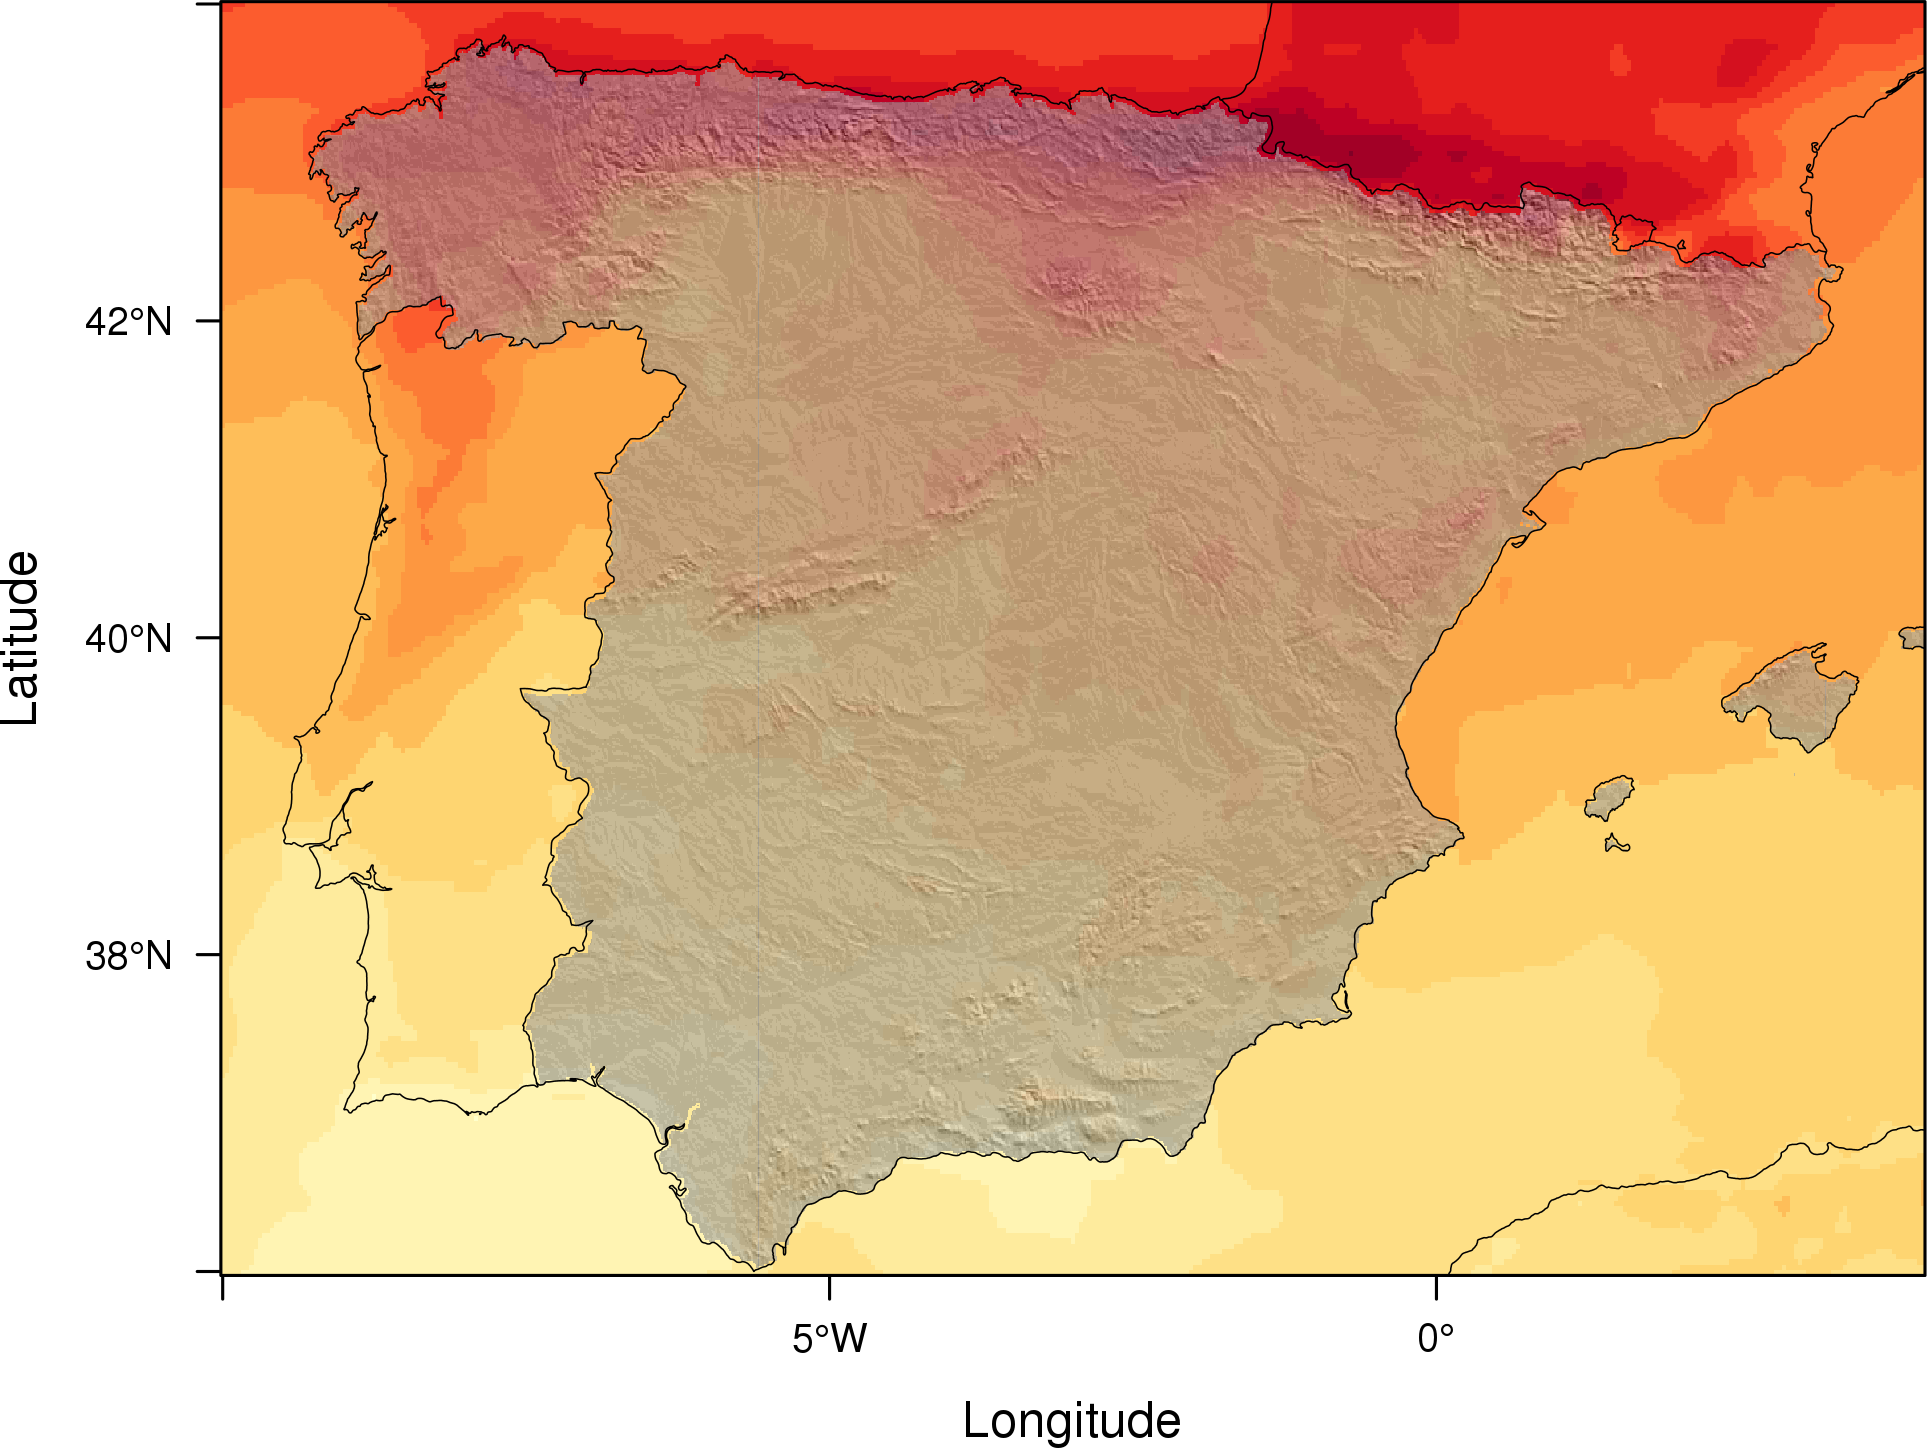
\includegraphics[width=.9\linewidth]{figs/hillShading.png}
\end{frame}

\subsection{3D}
\label{sec-2-4}

\begin{frame}[fragile,label=sec-2-4-1]{\texttt{plot3D} y \texttt{rgl}}
 \lstset{language=R,label= ,caption= ,numbers=none}
\begin{lstlisting}
  plot3D(DEM, maxpixels=5e4)
\end{lstlisting}

\begin{block}{}
El resultado puede exportarse en varios formatos tales como WebGL
usando \texttt{writeWebGL} (para un navegador), o \texttt{STL} con \texttt{writeSTL} para
impresión 3D. Este último formato se puede \href{https://github.com/oscarperpinan/spacetime-vis/blob/gh-pages/images/DEM.stl}{ver en GitHub}.

\lstset{language=R,label= ,caption= ,numbers=none}
\begin{lstlisting}
writeSTL('figs/DEM.stl')
\end{lstlisting}
\end{block}
\end{frame}

\section{Datos Categóricos}
\label{sec-3}

\subsection{Datos}
\label{sec-3-1}

\begin{frame}[fragile,label=sec-3-1-1]{NEO-NASA}
 \begin{itemize}
\item Uso del terreno
\begin{itemize}
\item \url{http://neo.sci.gsfc.nasa.gov/Search.html?group=20}
\end{itemize}
\item Densidad de población
\begin{itemize}
\item \url{http://neo.sci.gsfc.nasa.gov/Search.html?group=64}
\end{itemize}
\end{itemize}
\lstset{language=R,label= ,caption= ,numbers=none}
\begin{lstlisting}
  library(raster)
  ## China and India  
  ext <- extent(65, 135, 5, 55)
  
  pop <- raster('data/875430rgb-167772161.0.FLOAT.TIFF')
  pop <- crop(pop, ext)
  pop[pop==99999] <- NA
  
  landClass <- raster('data/241243rgb-167772161.0.TIFF')
  landClass <- crop(landClass, ext)
\end{lstlisting}
\end{frame}

\begin{frame}[fragile,label=sec-3-1-2]{RAT: \texttt{cut} y \texttt{ratify}}
 \lstset{language=R,label= ,caption= ,numbers=none}
\begin{lstlisting}
  landClass[landClass %in% c(0, 254)] <- NA
  ## Only four groups are needed:
  ## Forests: 1:5
  ## Shrublands, etc: 6:11
  ## Agricultural/Urban: 12:14
  ## Snow: 15:16
  landClass <- cut(landClass, c(0, 5, 11, 14, 16))
  ## Add a Raster Attribute Table and define the raster as categorical data
  landClass <- ratify(landClass)
  ## Configure the RAT: first create a RAT data.frame using the
  ## levels method; second, set the values for each class (to be
  ## used by levelplot); third, assign this RAT to the raster
  ## using again levels
  rat <- levels(landClass)[[1]]
  rat$classes <- c('Forest', 'Land', 'Urban', 'Snow')
  levels(landClass) <- rat
\end{lstlisting}
\end{frame}

\subsection{\texttt{levelplot}}
\label{sec-3-2}

\begin{frame}[fragile,label=sec-3-2-1]{Paleta de colores}
 \lstset{language=R,label= ,caption= ,numbers=none}
\begin{lstlisting}
  pal <- c('palegreen4', # Forest
           'lightgoldenrod', # Land
           'indianred4', # Urban
           'snow3')      # Snow
  
  catTheme <- modifyList(rasterTheme(),
                         list(panel.background = list(col='lightskyblue1'),
                              regions = list(col= pal)))
\end{lstlisting}
\end{frame}
\begin{frame}[fragile,label=sec-3-2-2]{}
 \lstset{language=R,label= ,caption= ,numbers=none}
\begin{lstlisting}
  levelplot(landClass, maxpixels=3.5e5, par.settings=catTheme,
            panel=panel.levelplot.raster)
\end{lstlisting}

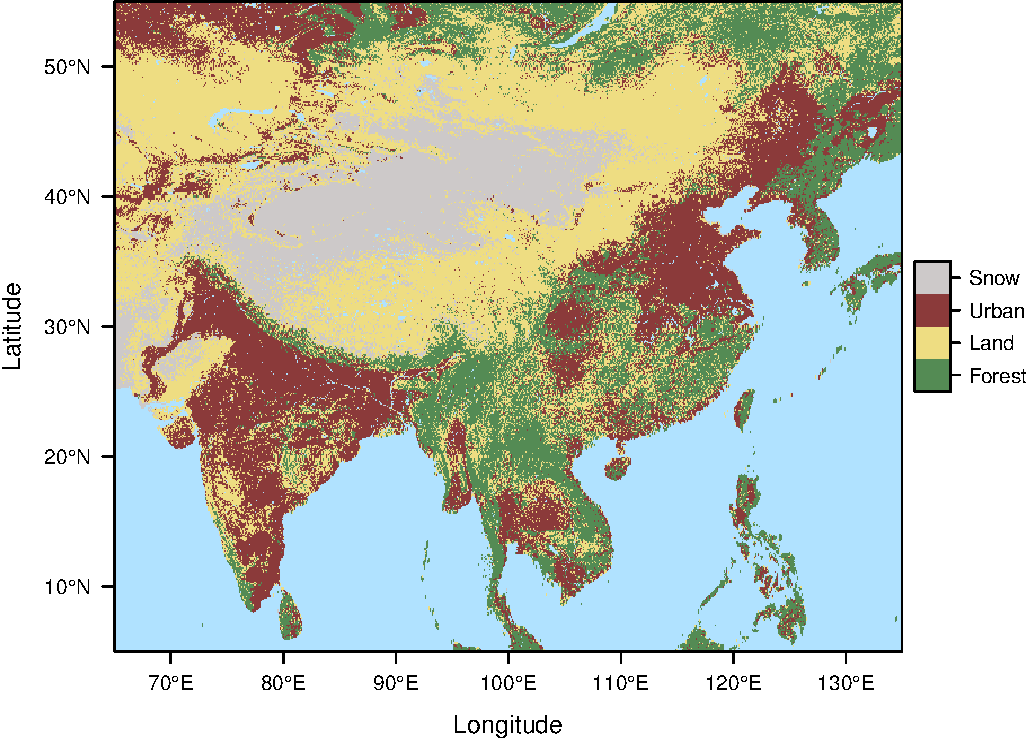
\includegraphics[width=.9\linewidth]{figs/landClass.pdf}
\end{frame}

\subsection{Datos cualitativos como variable de agrupación}
\label{sec-3-3}
\begin{frame}[fragile,label=sec-3-3-1]{Usamos cuantitativos como referencia}
 \lstset{language=R,label= ,caption= ,numbers=none}
\begin{lstlisting}
  pPop <- levelplot(pop, zscaleLog=10, par.settings=BTCTheme,
                    maxpixels=3.5e5, panel=panel.levelplot.raster)
  pPop
\end{lstlisting}

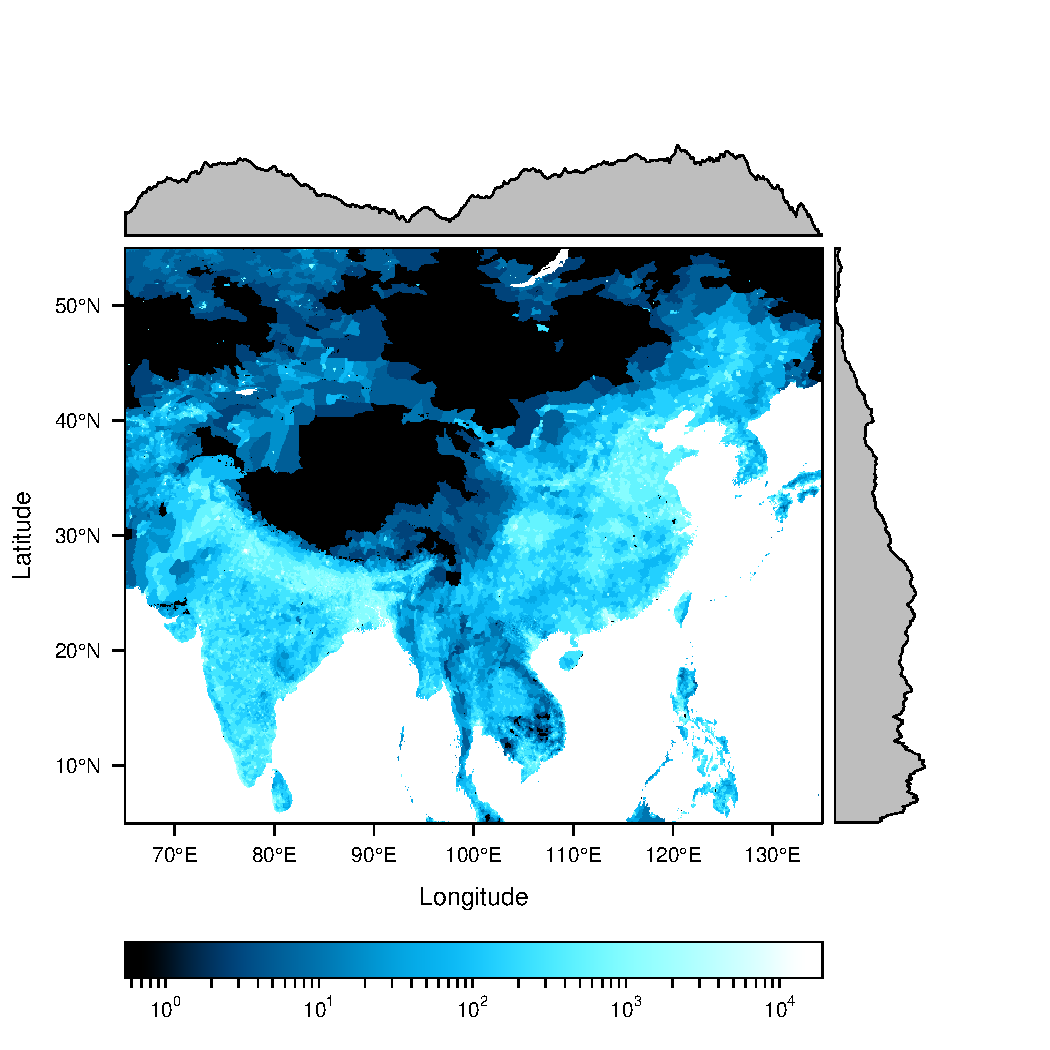
\includegraphics[width=.9\linewidth]{figs/populationNASA.pdf}
\end{frame}

\begin{frame}[fragile,label=sec-3-3-2]{Comparamos: histograma}
 \lstset{language=R,label= ,caption= ,numbers=none}
\begin{lstlisting}
  s <- stack(pop, landClass)
  names(s) <- c('pop', 'landClass')
  histogram(~log10(pop)|landClass, data=s,
            scales=list(relation='free'))
\end{lstlisting}

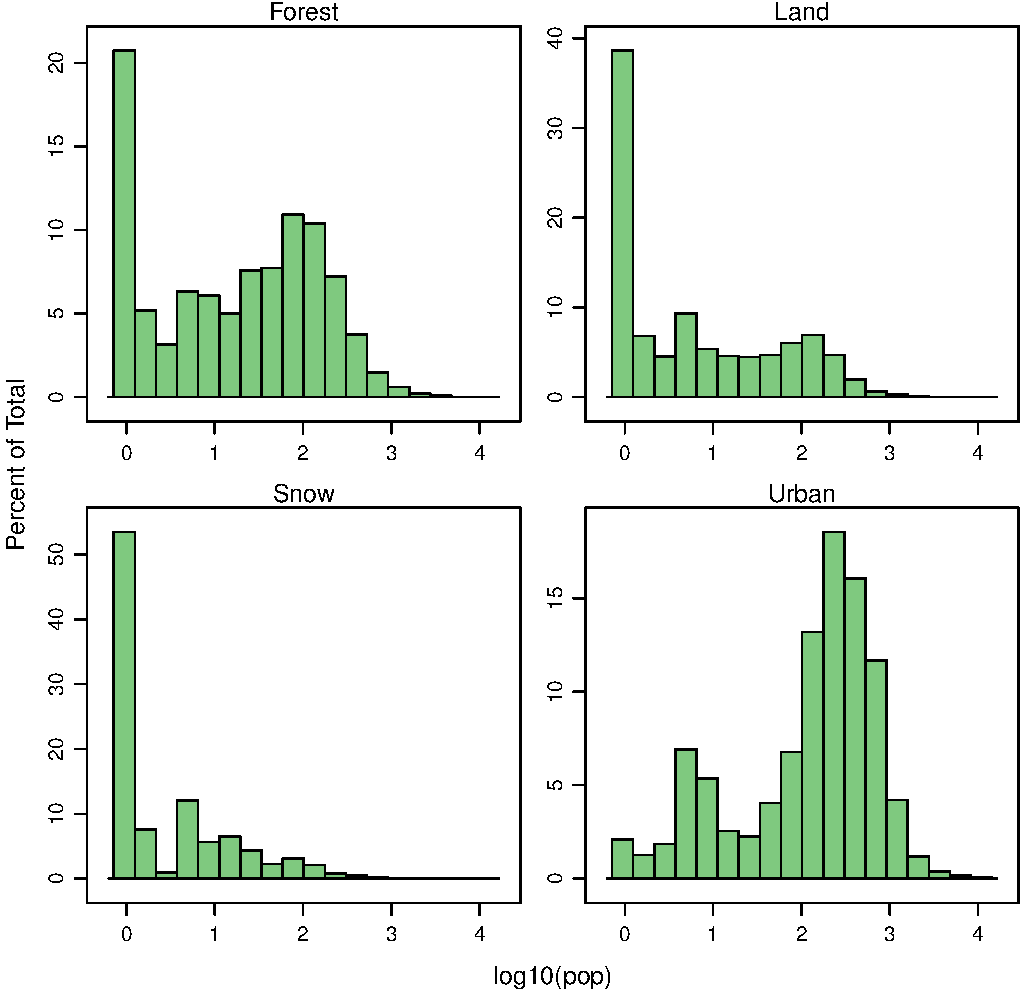
\includegraphics[width=.9\linewidth]{figs/histogramLandClass.pdf}
\end{frame}

\begin{frame}[fragile,label=sec-3-3-3]{Más comparaciones:}
 \begin{itemize}
\item \texttt{xyplot}
\item \texttt{densityplot}
\end{itemize}
\end{frame}

\section{Raster Espacio-Temporales}
\label{sec-4}

\subsection{Datos}
\label{sec-4-1}

\begin{frame}[fragile,label=sec-4-1-1]{Radiación solar en Galicia (2011)}
 \lstset{language=R,label= ,caption= ,numbers=none}
\begin{lstlisting}
  library(raster)
  library(zoo)
  library(rasterVis)
  
  SISdm <- brick('data/SISgal')
  
  timeIndex <- seq(as.Date('2011-01-01'), by='day', length=365)
  SISdm <- setZ(SISdm, timeIndex)
  names(SISdm) <- format(timeIndex, '%a_%Y%m%d')
\end{lstlisting}
\end{frame}


\subsection{Level Plots}
\label{sec-4-2}

\begin{frame}[fragile,label=sec-4-2-1]{Small multiple}
 \lstset{language=R,label= ,caption= ,numbers=none}
\begin{lstlisting}
  levelplot(SISdm, layers=1:12, panel=panel.levelplot.raster)
\end{lstlisting}


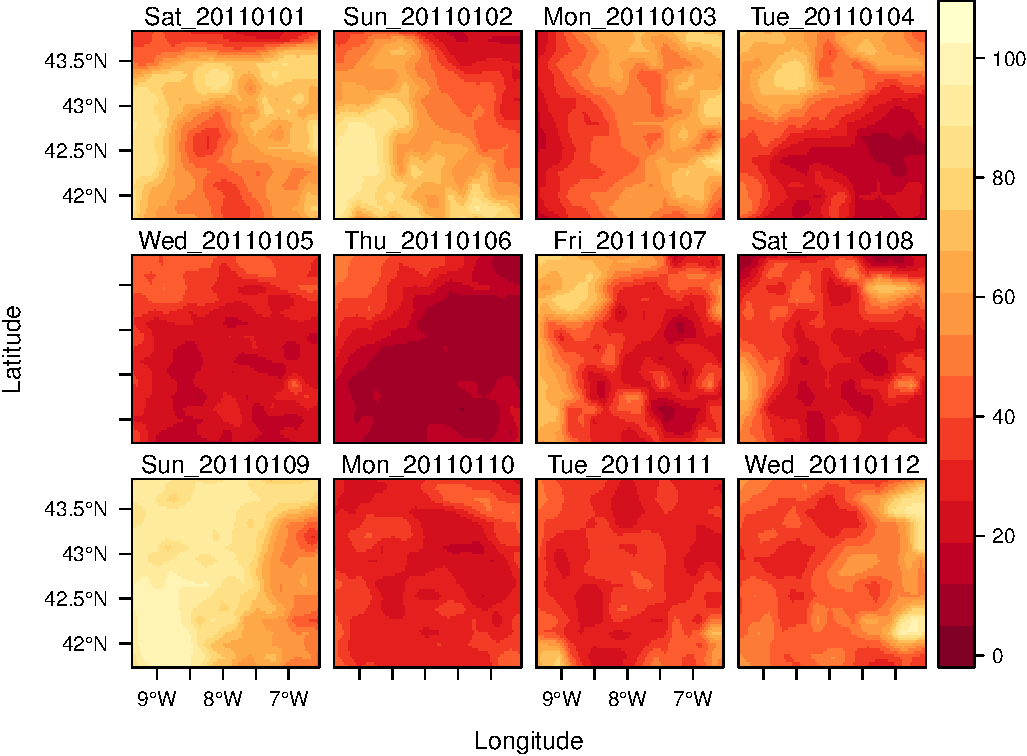
\includegraphics[width=.9\linewidth]{figs/SISdm.pdf}
\end{frame}

\begin{frame}[fragile,label=sec-4-2-2]{Reducimos número de capas: \texttt{zApply}}
 \lstset{language=R,label= ,caption= ,numbers=none}
\begin{lstlisting}
  SISmm <- zApply(SISdm, by=as.yearmon, fun='mean')
\end{lstlisting}

\lstset{language=R,label= ,caption= ,numbers=none}
\begin{lstlisting}
  levelplot(SISmm, panel=panel.levelplot.raster)
\end{lstlisting}

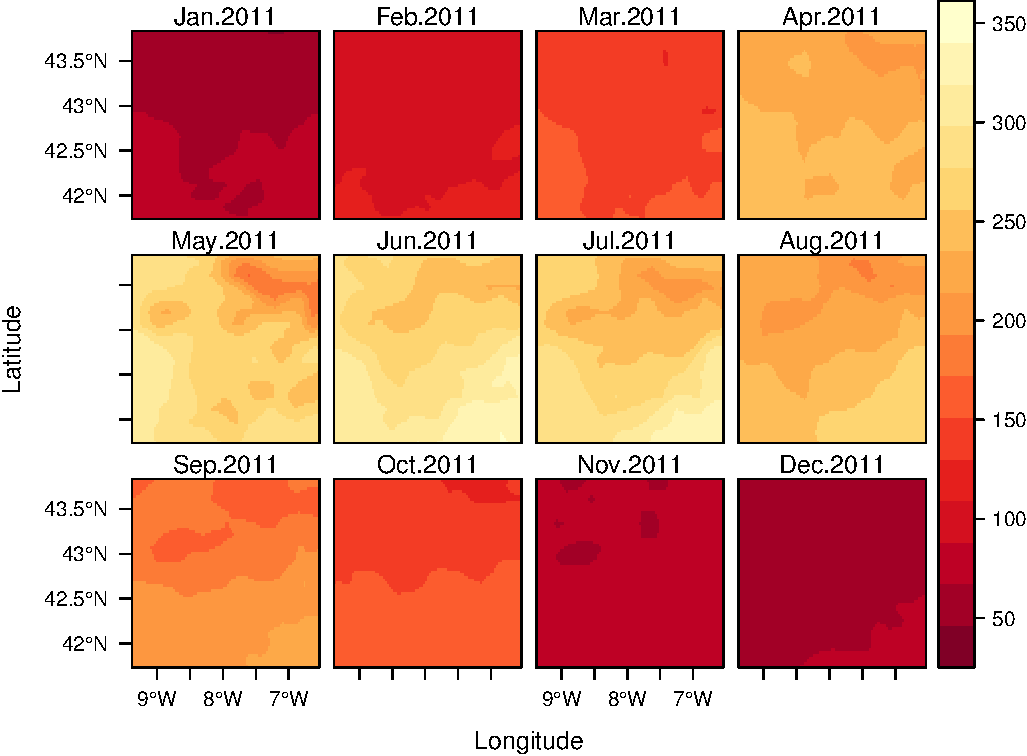
\includegraphics[width=.9\linewidth]{figs/SISmm.pdf}
\end{frame}

\subsection{Gráficos EDA (Exploratory Data Analysis)}
\label{sec-4-3}


\begin{frame}[fragile,label=sec-4-3-1]{Histograma}
 \lstset{language=R,label= ,caption= ,numbers=none}
\begin{lstlisting}
  histogram(SISdm, FUN=as.yearmon)
\end{lstlisting}

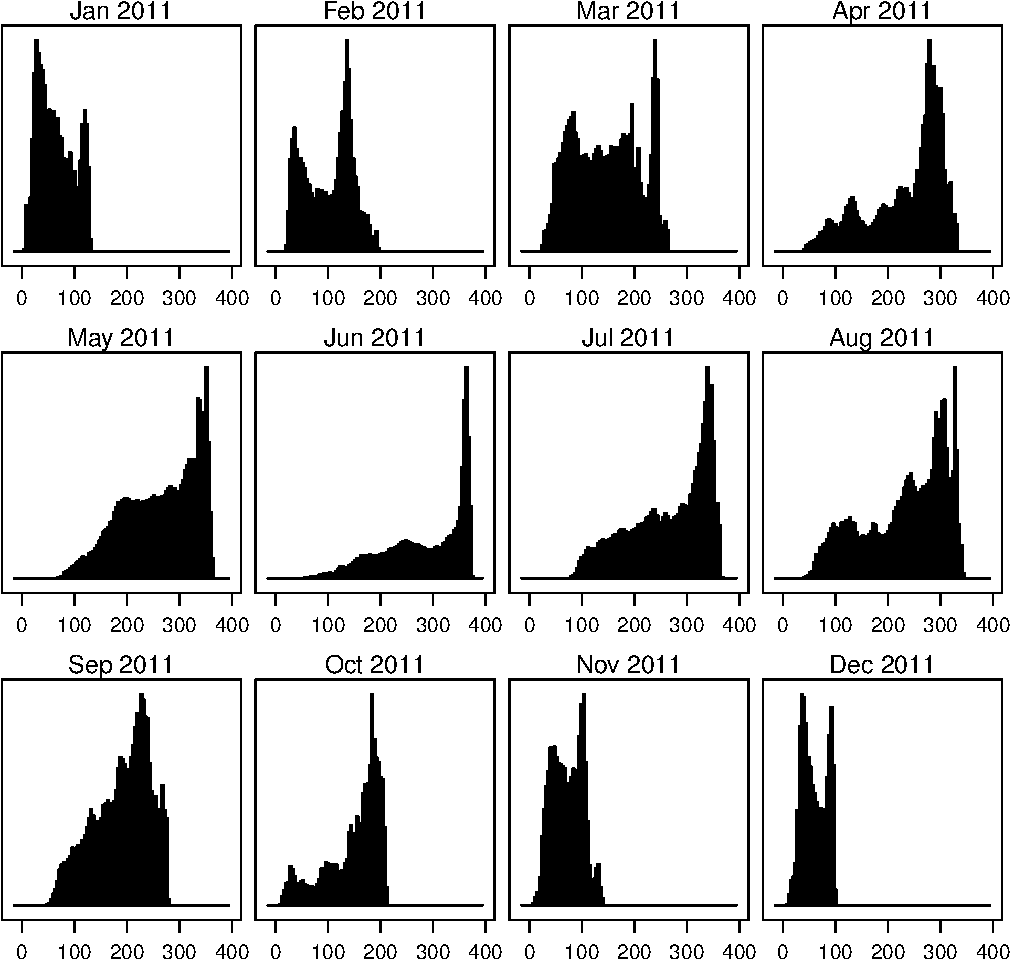
\includegraphics[width=.9\linewidth]{figs/SISdm_histogram.pdf}
\end{frame}

\begin{frame}[fragile,label=sec-4-3-2]{Violin plot}
 \lstset{language=R,label= ,caption= ,numbers=none}
\begin{lstlisting}
  bwplot(SISdm, FUN=as.yearmon)
\end{lstlisting}

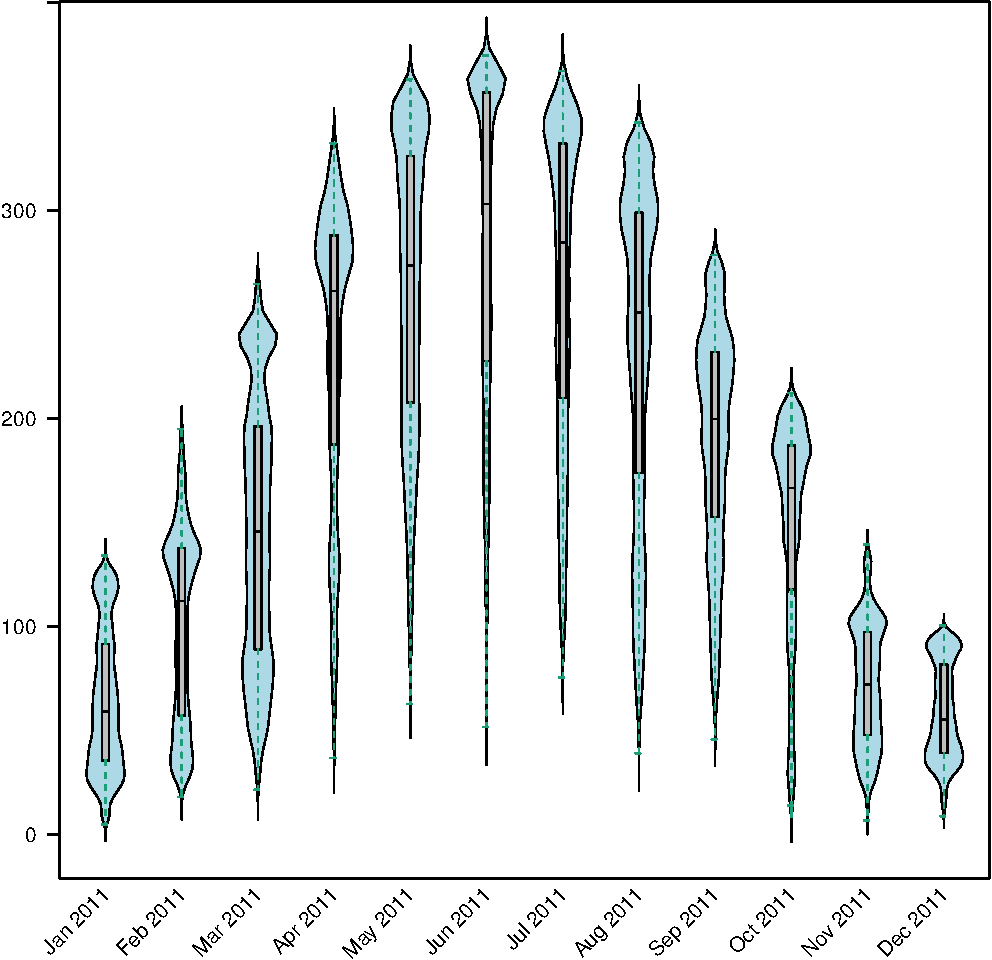
\includegraphics[width=.9\linewidth]{figs/SISdm_boxplot.pdf}
\end{frame}

\begin{frame}[fragile,label=sec-4-3-3]{Matriz de gráficos de dispersión}
 \lstset{language=R,label= ,caption= ,numbers=none}
\begin{lstlisting}
  splom(SISmm, xlab='', plot.loess=TRUE)
\end{lstlisting}

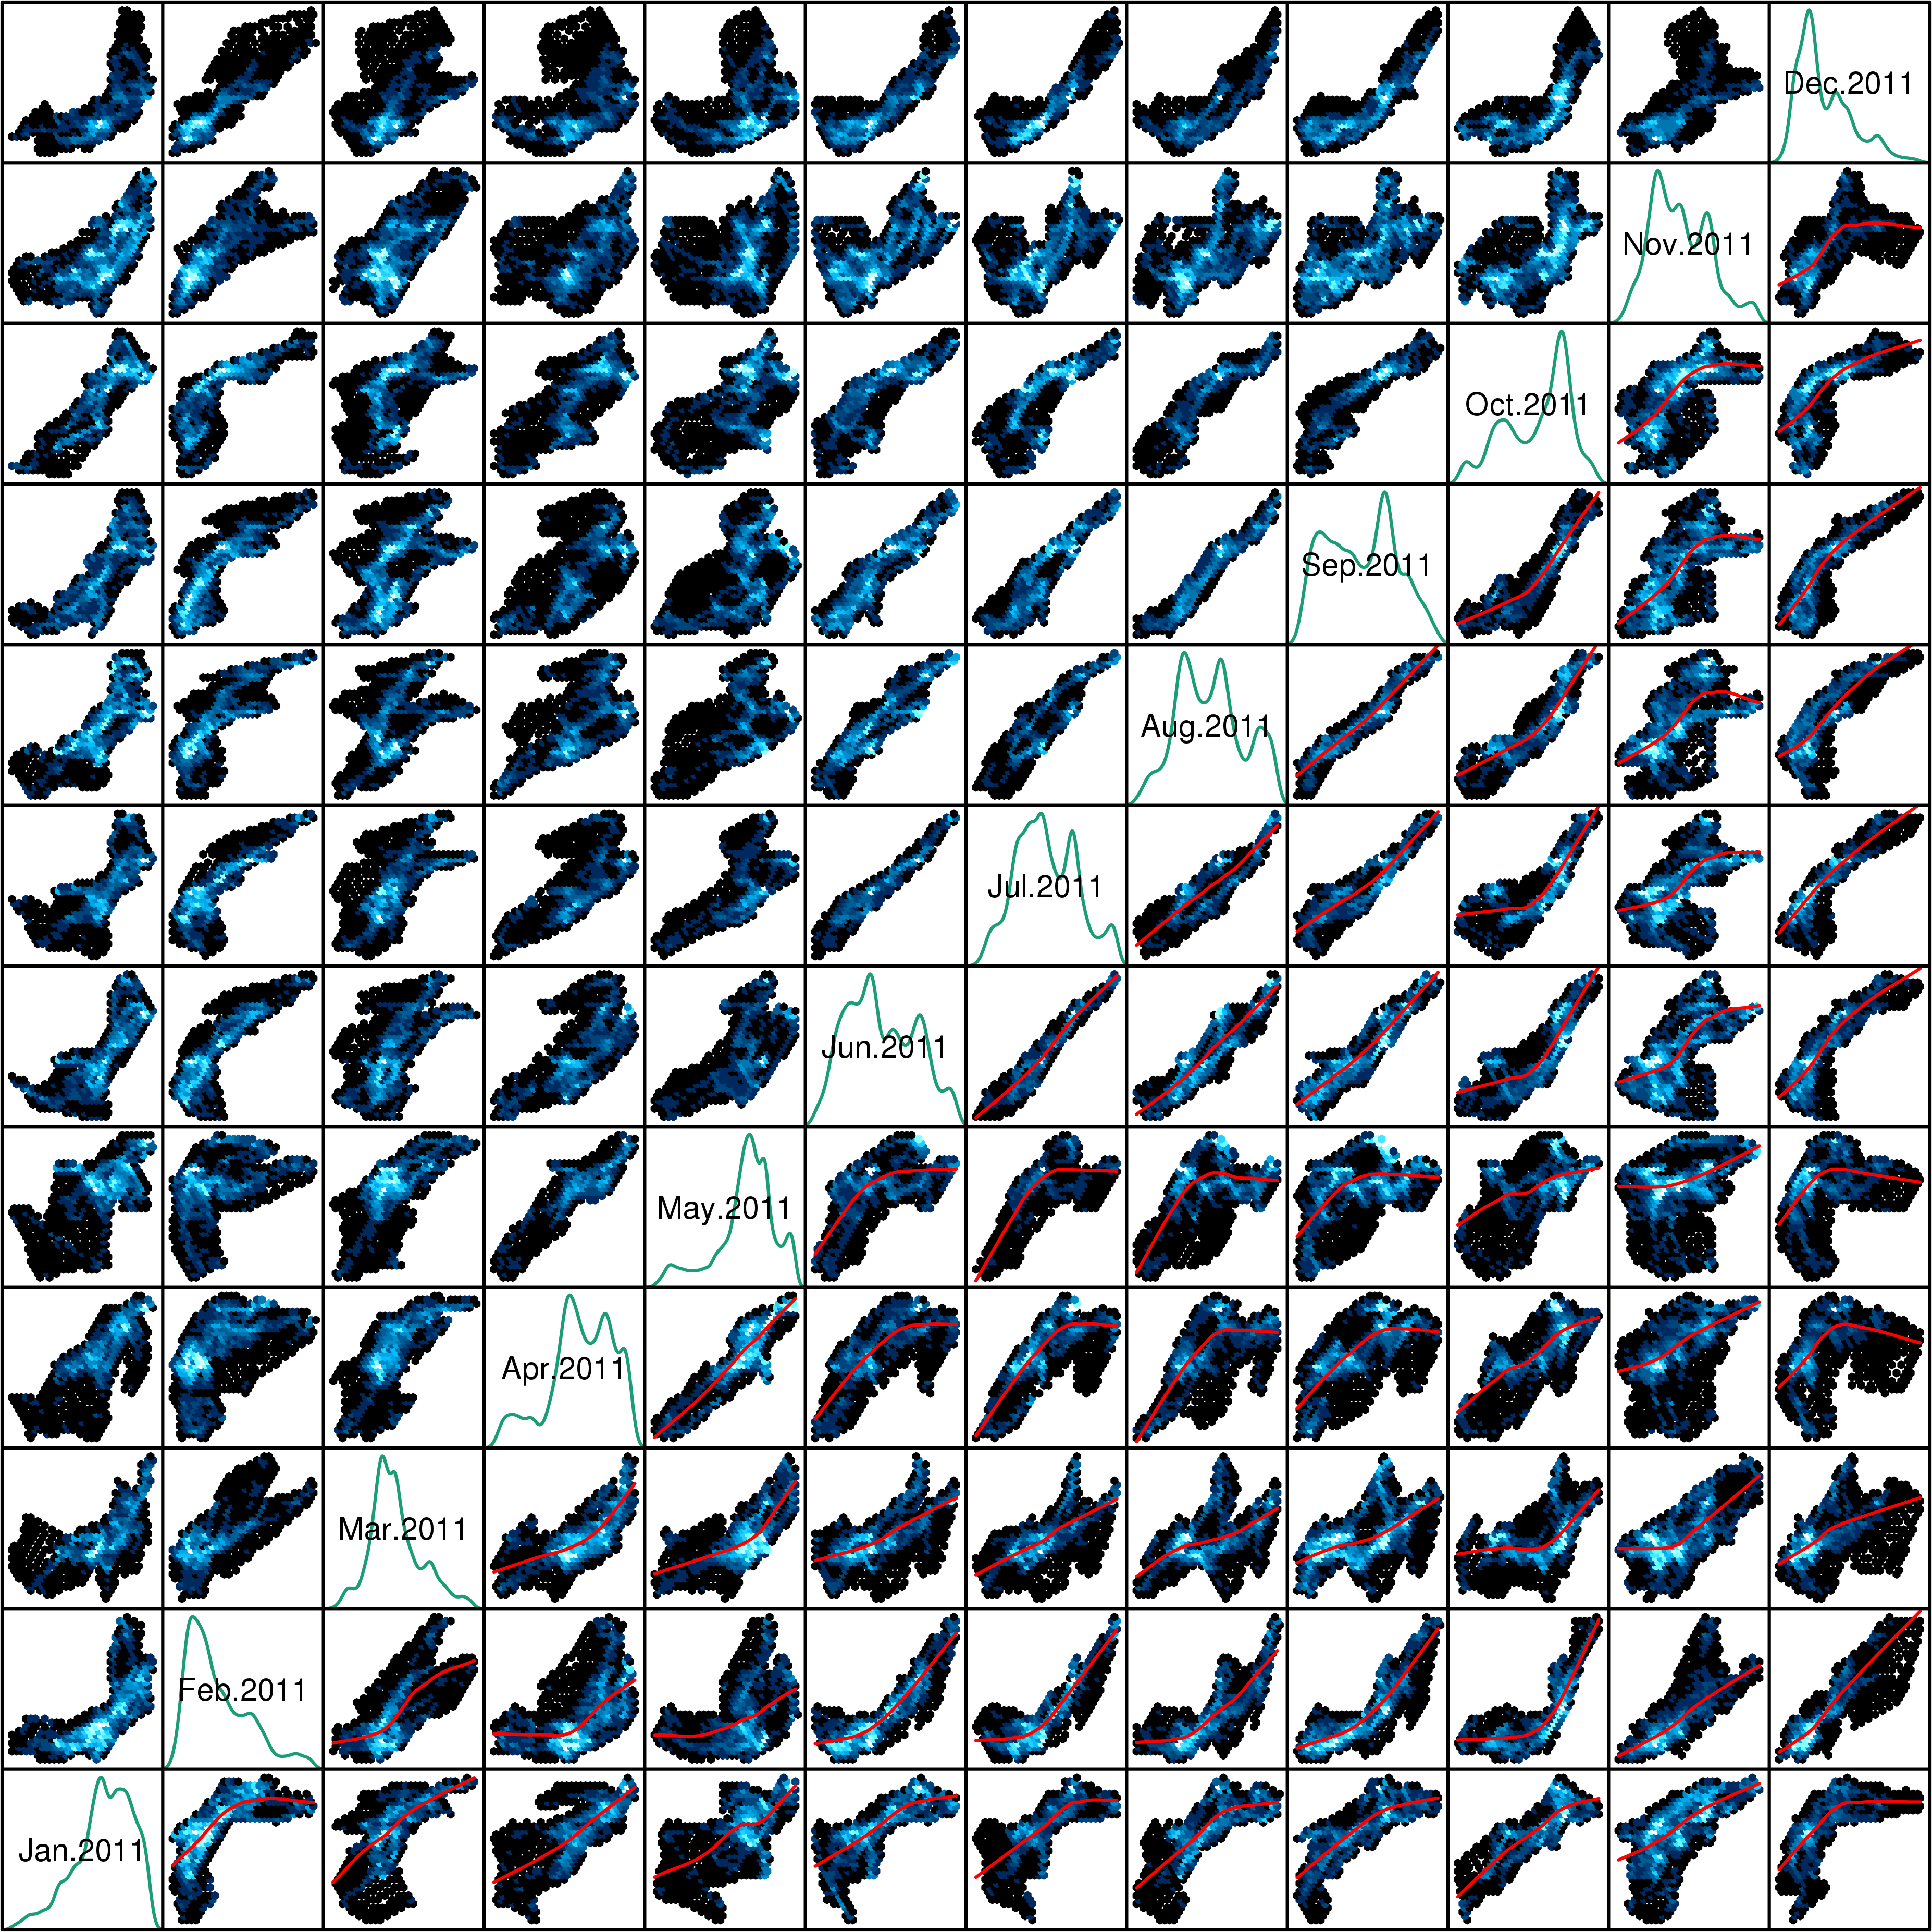
\includegraphics[width=.9\linewidth]{figs/SISmm_splom.png}
\end{frame}


\subsection{Gráficos espacio temporales}
\label{sec-4-4}

\begin{frame}[fragile,label=sec-4-4-1]{Hovmoller}
 \lstset{language=R,label= ,caption= ,numbers=none}
\begin{lstlisting}
  hovmoller(SISdm, par.settings=BTCTheme())
\end{lstlisting}
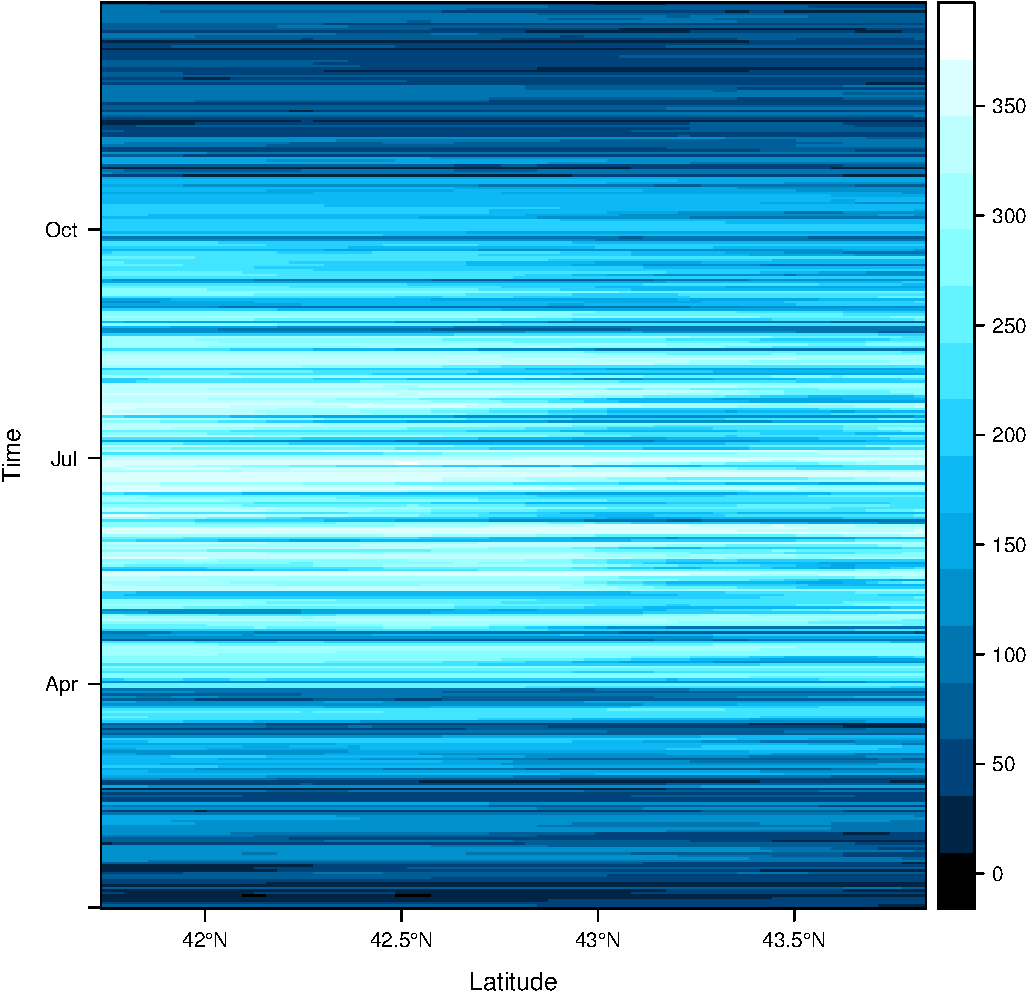
\includegraphics[width=.9\linewidth]{figs/SISdm_hovmoller_lat.pdf}
\end{frame}

\begin{frame}[fragile,label=sec-4-4-2]{xyplot}
 \lstset{language=R,label= ,caption= ,numbers=none}
\begin{lstlisting}
  xyplot(SISdm, digits=1, col='black', lwd=0.2, alpha=0.6)
\end{lstlisting}

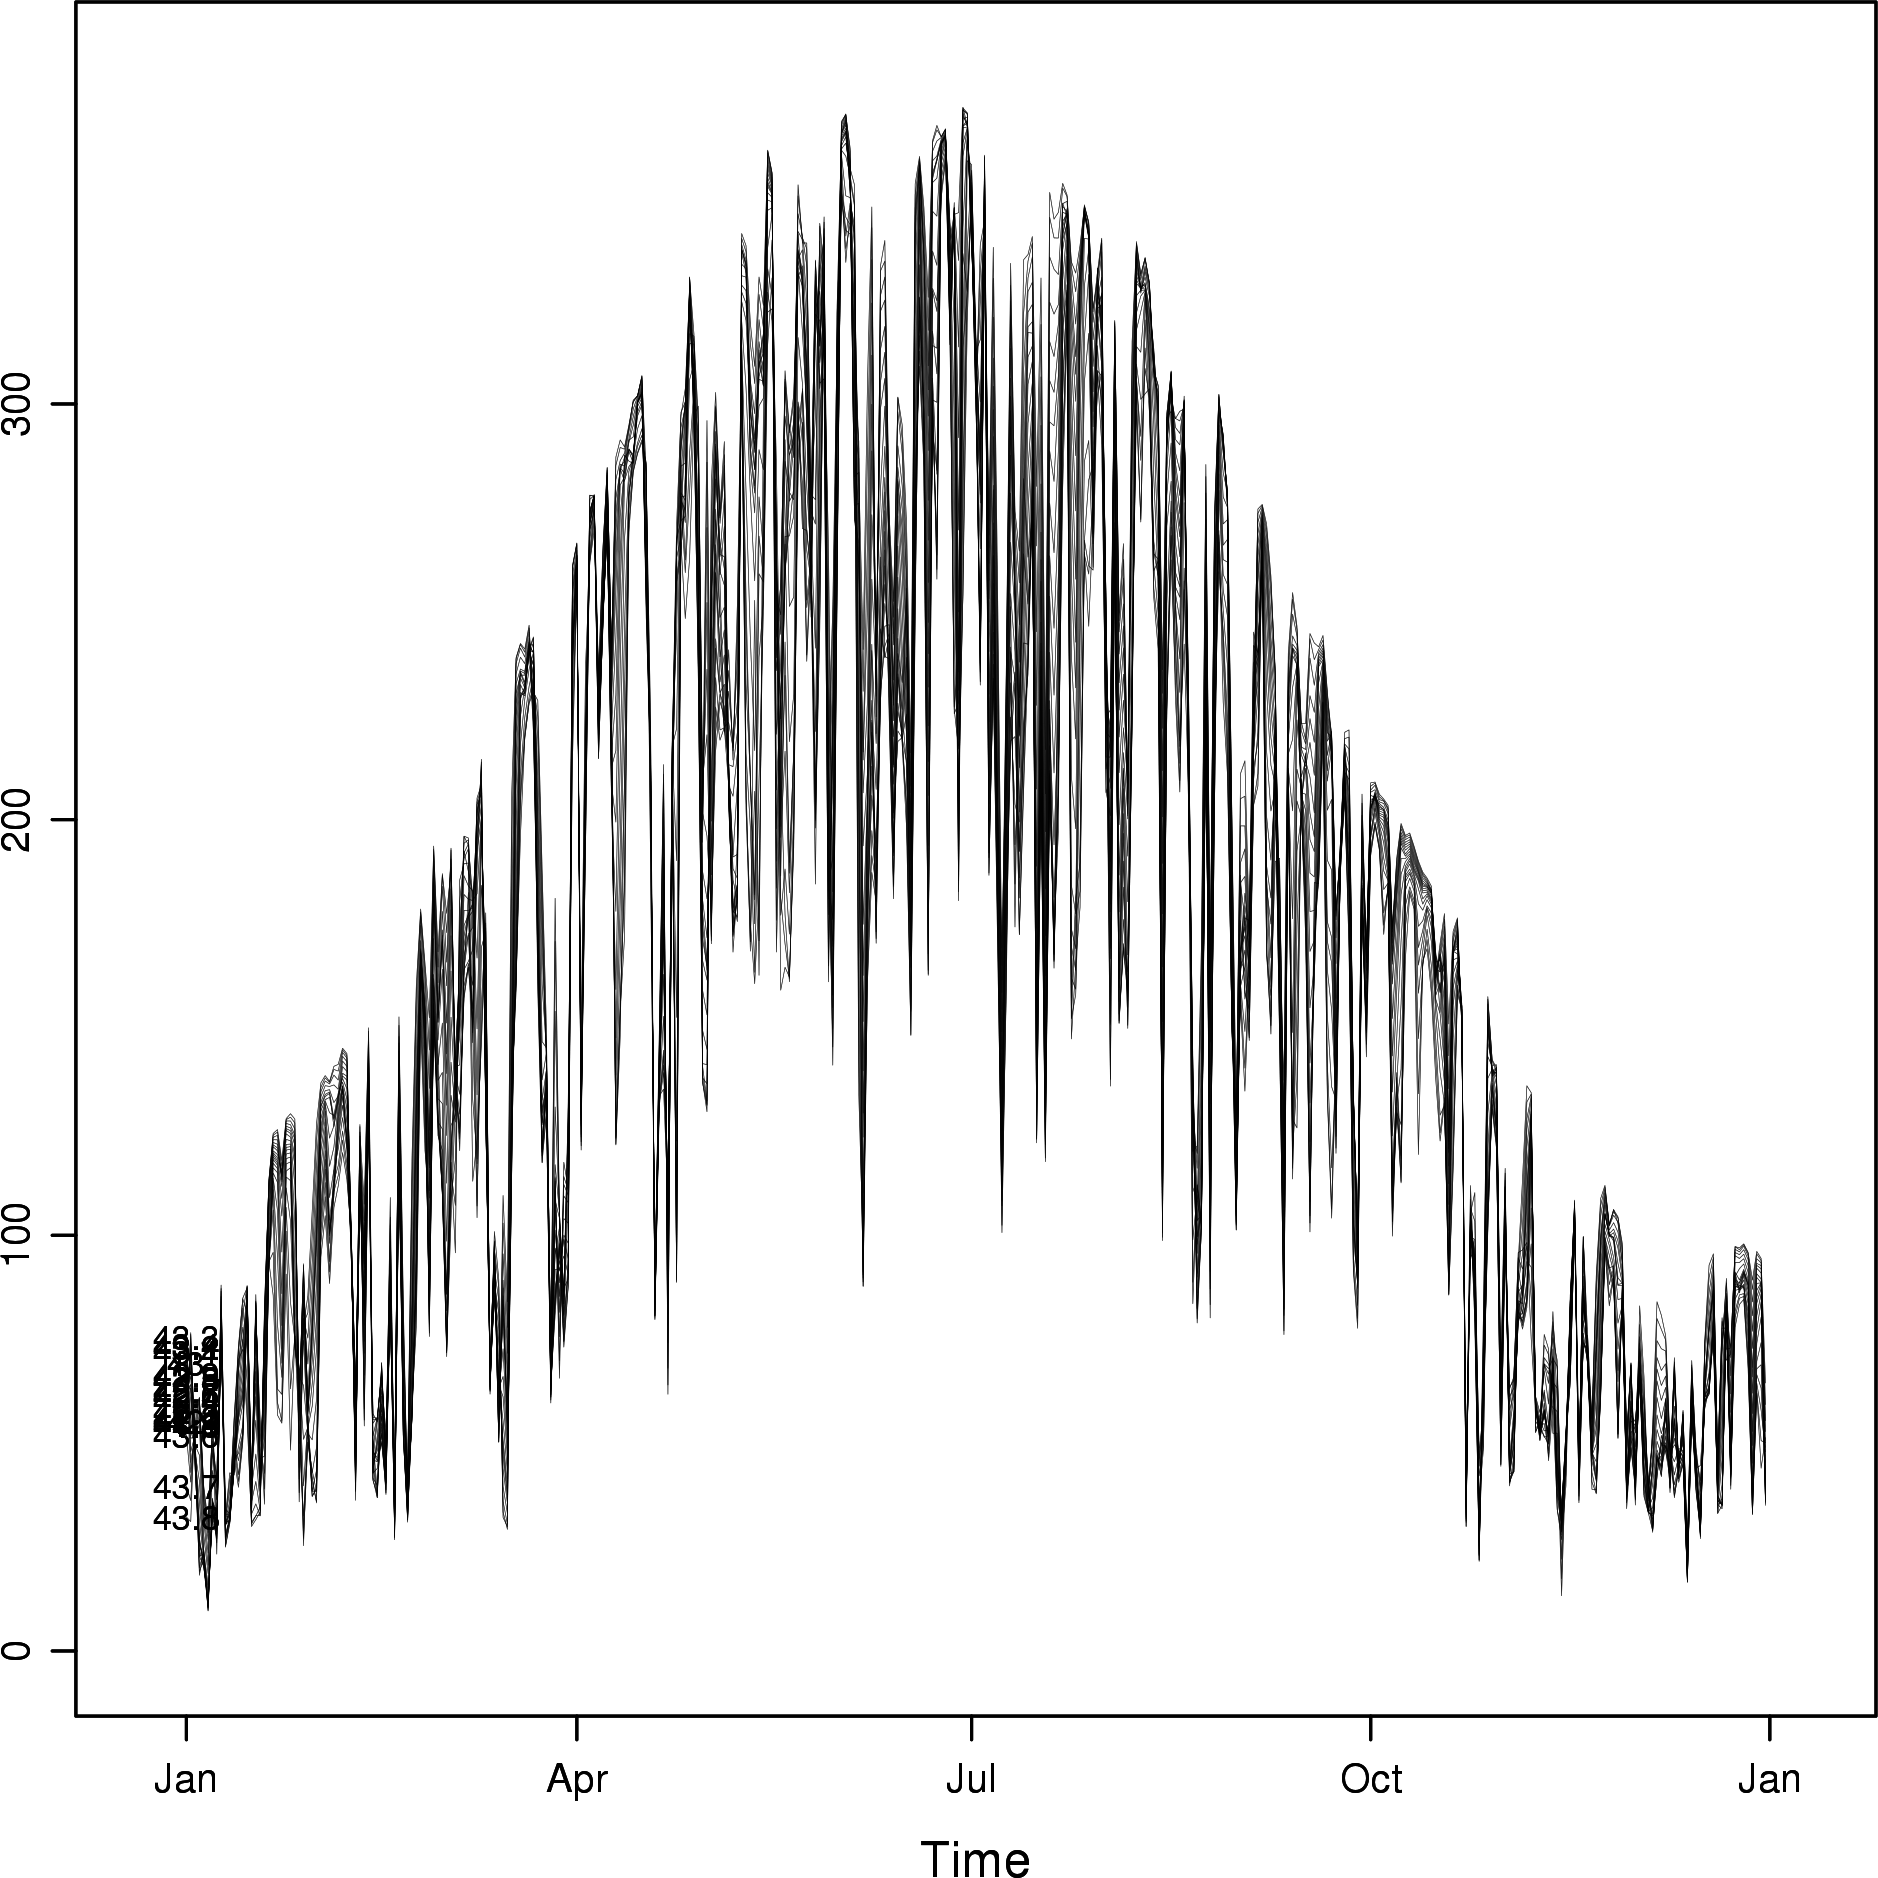
\includegraphics[width=.9\linewidth]{figs/SISmm_xyplot.png}
\end{frame}

\begin{frame}[fragile,label=sec-4-4-3]{Horizonplot}
 \lstset{language=R,label= ,caption= ,numbers=none}
\begin{lstlisting}
  horizonplot(SISdm, digits=1,
              col.regions=rev(brewer.pal(n=6, 'PuOr')),
              xlab='', ylab='Latitude')
\end{lstlisting}

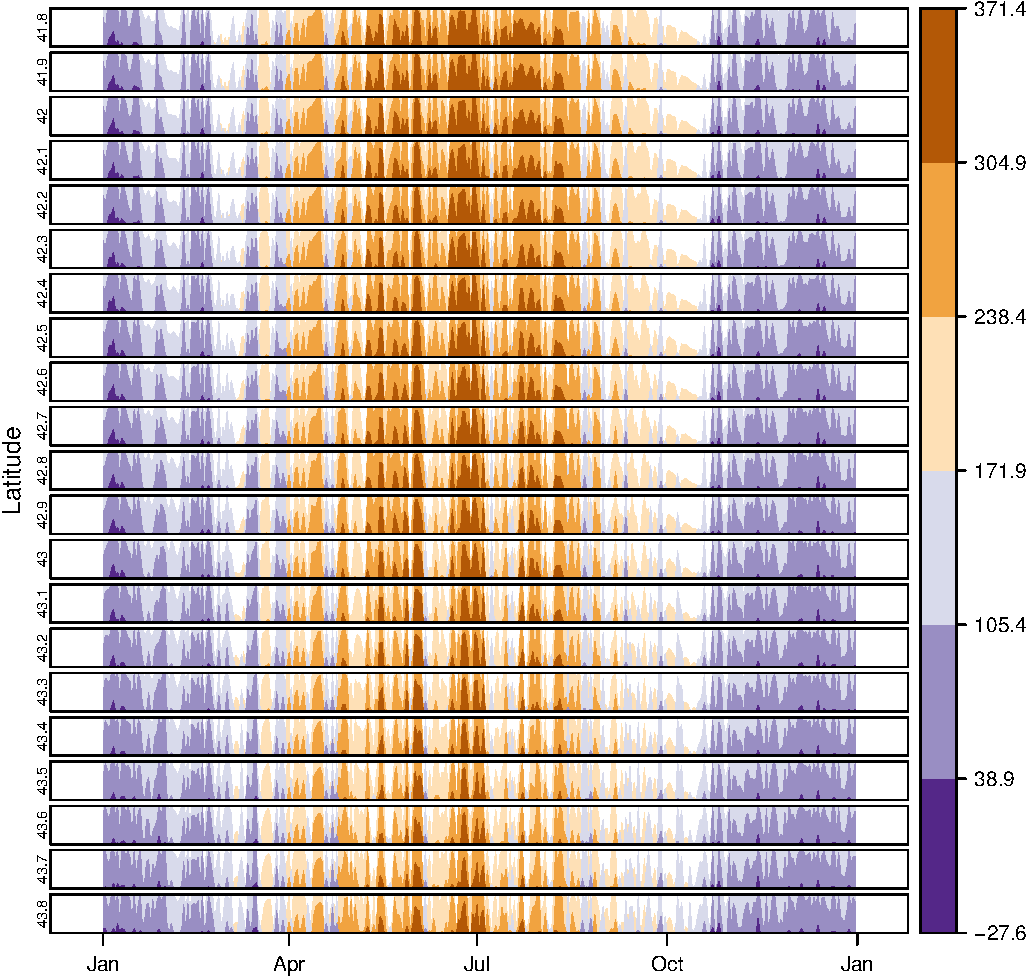
\includegraphics[width=.9\linewidth]{figs/SISdm_horizonplot.pdf}
\end{frame}


\subsection{Animación}
\label{sec-4-5}

\begin{frame}[fragile,label=sec-4-5-1]{Datos de Meteogalicia}
 \begin{itemize}
\item Predicción horaria de cobertura nubosa
\end{itemize}
\lstset{language=R,label= ,caption= ,numbers=none}
\begin{lstlisting}
  cft <- brick('data/cft_20130417_0000.nc')
  ## use memory instead of file
  cft[] <- getValues(cft)
  ## set projection
  projLCC2d <- "+proj=lcc +lon_0=-14.1 +lat_0=34.823 +lat_1=43 +lat_2=43 +x_0=536402.3 +y_0=-18558.61 +units=km +ellps=WGS84"
  projection(cft) <- projLCC2d
  #set time index
  timeIndex <- seq(as.POSIXct('2013-04-17 01:00:00', tz='UTC'), length=96, by='hour')
  cft <- setZ(cft, timeIndex)
  names(cft) <- format(timeIndex, 'D%d_H%H')
\end{lstlisting}

\begin{block}{\url{http://mandeo.meteogalicia.es/thredds/catalogos/WRF_2D/catalog.html}}
\end{block}
\end{frame}


\begin{frame}[fragile,label=sec-4-5-2]{Referencia espacial: fronteras administrativas}
 \lstset{language=R,label= ,caption= ,numbers=none}
\begin{lstlisting}
  library(maptools)
  library(rgdal)
  library(maps)
  library(mapdata)
  
  
  projLL <- CRS('+proj=longlat +datum=WGS84 +ellps=WGS84 +towgs84=0,0,0')
  cftLL <- projectExtent(cft, projLL)
  cftExt <- as.vector(bbox(cftLL))
  boundaries <- map('worldHires',
                    xlim=cftExt[c(1,3)], ylim=cftExt[c(2,4)],
                    plot=FALSE)
  boundaries <- map2SpatialLines(boundaries, proj4string=projLL)
  boundaries <- spTransform(boundaries, CRS(projLCC2d))
\end{lstlisting}
\end{frame}


\begin{frame}[fragile,label=sec-4-5-3]{Generamos imágenes para una película}
 \begin{itemize}
\item Definimos la paleta de colores
\end{itemize}
\lstset{language=R,label= ,caption= ,numbers=none}
\begin{lstlisting}
  cloudTheme <- rasterTheme(region=brewer.pal(n=9, 'Blues'))
\end{lstlisting}

\begin{itemize}
\item Con \texttt{layout(1, 1)} generamos un fichero por cada capa.
\end{itemize}
\lstset{language=R,label= ,caption= ,numbers=none}
\begin{lstlisting}
  tmp <- tempdir()
  trellis.device(png, file=paste0(tmp, '/Rplot%02d.png'),
                        res=300, width=1500, height=1500)
  levelplot(cft, layout=c(1, 1), par.settings=cloudTheme) +
      layer(sp.lines(boundaries, lwd=0.6))
  dev.off()
\end{lstlisting}
\end{frame}

\begin{frame}[fragile,label=sec-4-5-4]{Componemos la película con ffmpeg}
 \lstset{language=R,label= ,caption= ,numbers=none}
\begin{lstlisting}
  old <- setwd(tmp)
  ## Create a movie with ffmpeg using 6 frames per second a bitrate of 300kbs
  movieCMD <- 'ffmpeg -r 6 -b 300k -i Rplot%02d.png output.mp4'
  system(movieCMD)
  file.remove(dir(pattern='Rplot'))
  file.copy('output.mp4', paste0(old, '/figs/cft.mp4'), overwrite=TRUE)
  setwd(old)
\end{lstlisting}

\begin{block}{}
\href{http://vimeo.com/user18057623/cft}{Video}
\end{block}
\end{frame}

\begin{frame}[fragile,label=sec-4-5-5]{Como referencia: small multiple}
 \lstset{language=R,label= ,caption= ,numbers=none}
\begin{lstlisting}
  levelplot(cft, layers=25:48, layout=c(6, 4),
            par.settings=cloudTheme,
            names.attr=paste0(sprintf('%02d', 1:24), 'h'),
            panel=panel.levelplot.raster) +
      layer(sp.lines(boundaries, lwd=0.6))
\end{lstlisting}

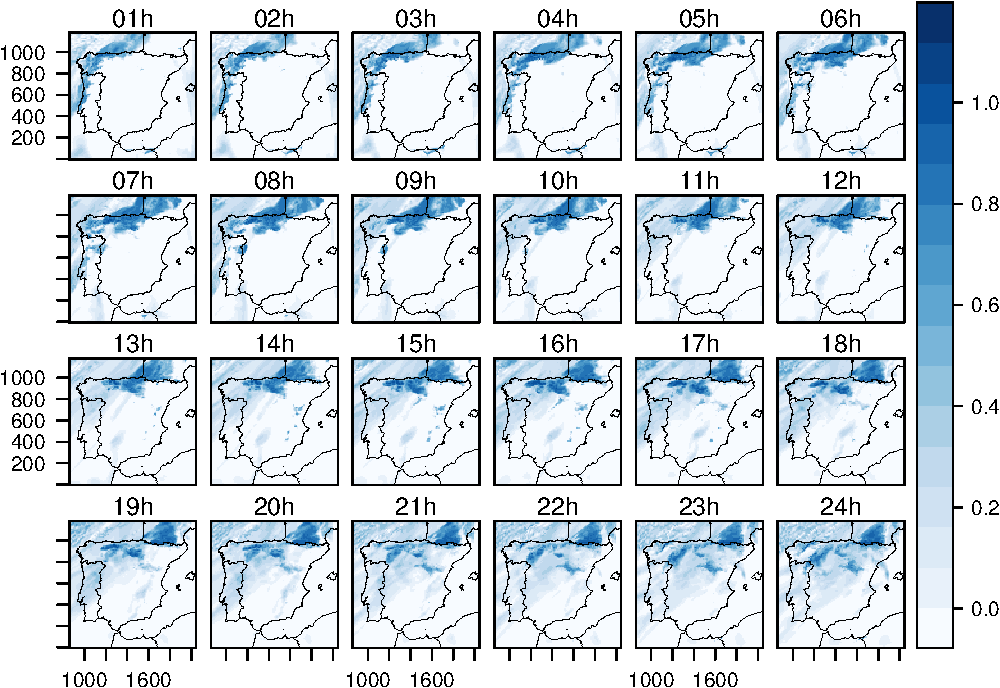
\includegraphics[width=.9\linewidth]{figs/cft.pdf}
\end{frame}


\section{Campos Vectoriales}
\label{sec-5}

\subsection{Datos}
\label{sec-5-1}

\begin{frame}[fragile,label=sec-5-1-1]{Predicciones de viento de Meteogalicia}
 \lstset{language=R,label= ,caption= ,numbers=none}
\begin{lstlisting}
  library(raster)
  library(rasterVis)
  
  wDir <- raster('data/wDir')/180*pi
  wSpeed <- raster('data/wSpeed')
  windField <- stack(wSpeed, wDir)
  names(windField) <- c('magnitude', 'direction')
\end{lstlisting}
\end{frame}


\subsection{Gráficos de flechas}
\label{sec-5-2}
\begin{frame}[fragile,label=sec-5-2-1]{\texttt{vectorplot}}
 \begin{itemize}
\item En puntos discretos (muestreando el raster) se dibuja una flecha con dirección y sentido las del campo en ese punto, y con una longitud proporcional a la magnitud del campo.
\end{itemize}

\lstset{language=R,label= ,caption= ,numbers=none}
\begin{lstlisting}
  vectorplot(windField, isField=TRUE, par.settings=BTCTheme(),
             colorkey=FALSE, scales=list(draw=FALSE))
\end{lstlisting}
\end{frame}

\begin{frame}[label=sec-5-2-2]{}
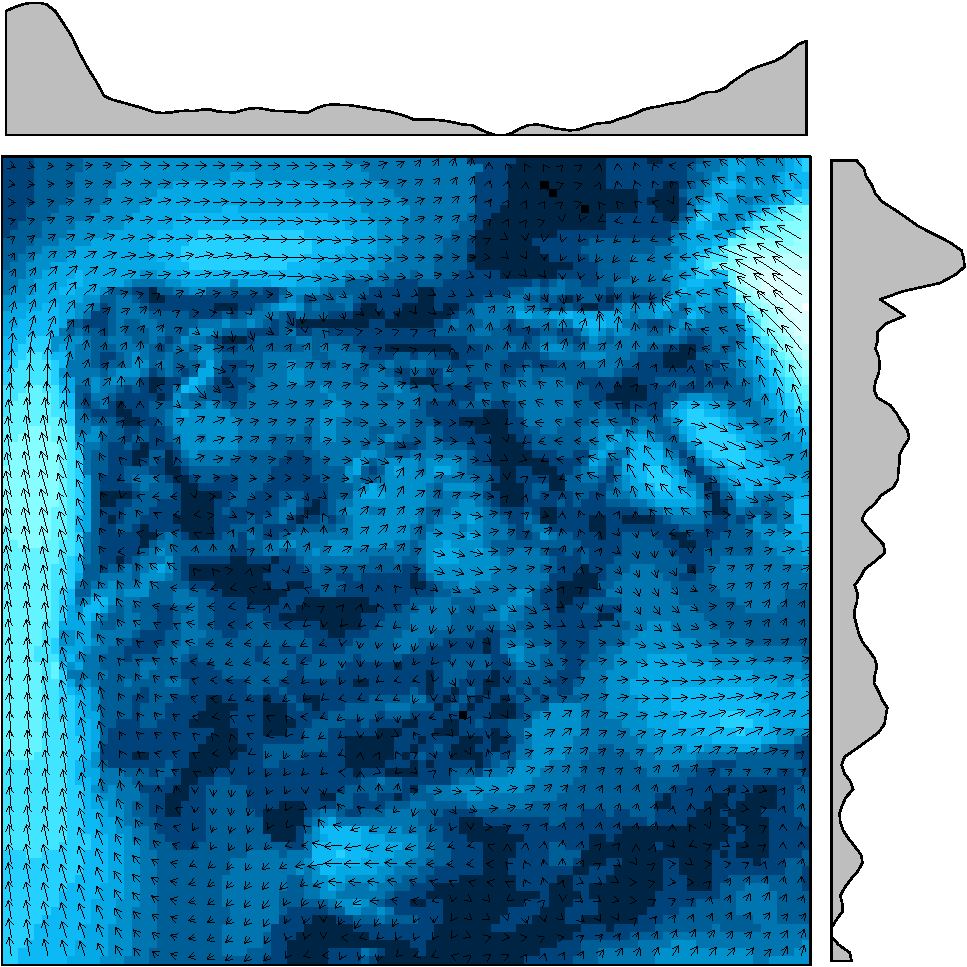
\includegraphics[width=.9\linewidth]{figs/vectorplot.pdf}
\end{frame}

\subsection{Streamlines}
\label{sec-5-3}
\begin{frame}[label=sec-5-3-1]{FROLIC}
\begin{itemize}
\item Curvas integrales, líneas de flujo (\emph{streamlines}).
\item Algoritmo (adaptado de \href{https://www.cg.tuwien.ac.at/research/vis-dyn-syst/frolic/frolic_crc.pdf}{FROLIC}):
\begin{itemize}
\item En cada punto (\emph{droplet}) de una
rejilla regular, se calcula una pequeña porción de la línea de
flujo (\emph{streamlet}) integrando el campo vectorial en ese punto.
\item El color principal de cada \emph{streamlet} indica la magnitud local del campo.
\item Cada \emph{streamlet} está compuesta por puntos cuyos tamaños,
posición, y degradación, codifican la dirección local del campo.
\end{itemize}
\end{itemize}
\end{frame}

\begin{frame}[fragile,label=sec-5-3-2]{\texttt{streamplot}}
 \lstset{language=R,label= ,caption= ,numbers=none}
\begin{lstlisting}
  myTheme <- streamTheme(region=rev(brewer.pal(n=4, name='Greys')),
                                      symbol=BTC(n=9, beg=20))
  streamplot(windField, isField=TRUE,
             par.settings=myTheme,
             droplet=list(pc=12),
             streamlet=list(L=5, h=5),
             scales=list(draw=FALSE),
             panel=panel.levelplot.raster)
\end{lstlisting}
\end{frame}

\begin{frame}[label=sec-5-3-3]{}
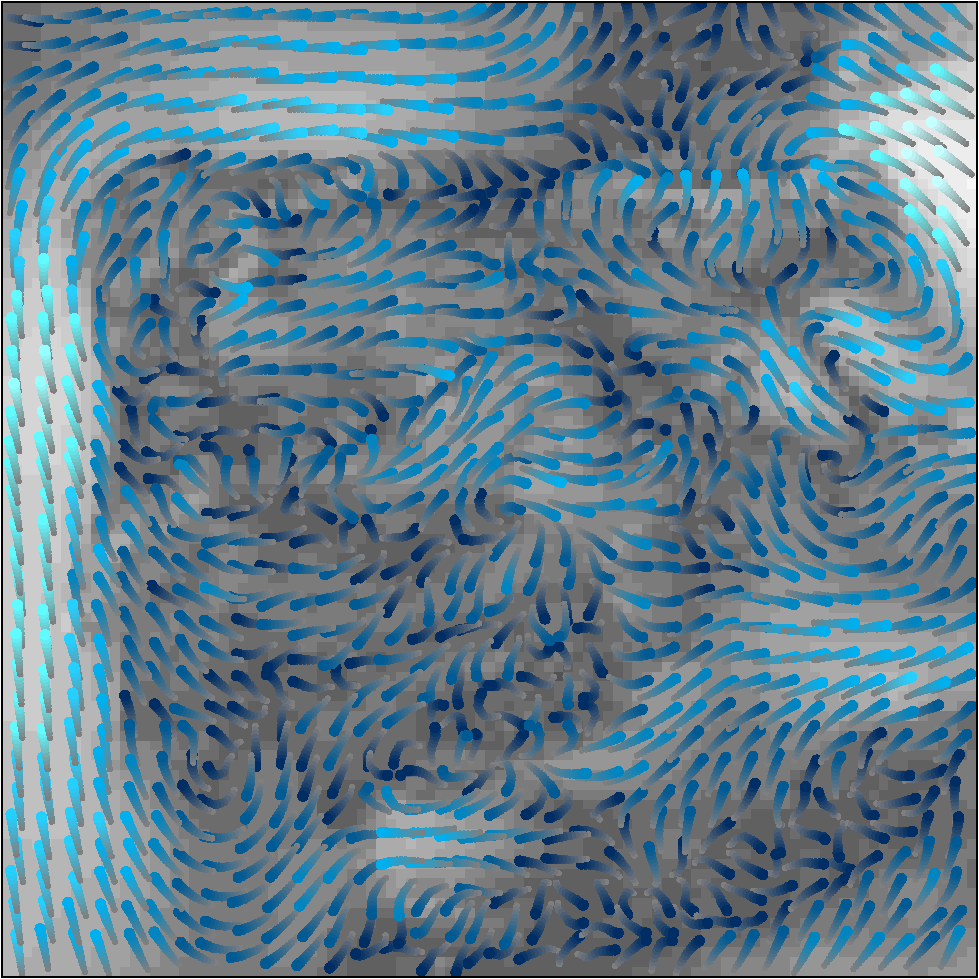
\includegraphics[width=.9\linewidth]{figs/streamplot.pdf}
\end{frame}

\begin{frame}[label=sec-5-3-4]{Tu turno}

\end{frame}
% Emacs 24.3.1 (Org mode 8.2.7c)
\end{document}